\chapter{Leistungsendstufen}

In diesem Kapitel werden Leistungsendstufen mit zwei komplementären Transistoren behandelt.

\section{Übernahmeverzerrung}

\begin{figure}[H]
    \centering
    \includegraphics[width = \textwidth]{simulations/7_Leistungsendstufe/Übernahmeverzerrungen.pdf}
    \caption{Übernahmeverzerrungen}
    \label{fig:my_label}
\end{figure}

Trotz der Unterschiede in der Wellenform, waren für mich bei einer Grundfrequenz von \SI{1}{\hilo \hertz} keine Unterschiede hörbar.

Im Frequenzspektrum betrachtet, wirken sich diese nicht-Linearitäten  in der Verstärkung wie folgt aus:

\begin{figure}[H]
    \centering
    \includegraphics[width = \textwidth]{simulations/7_Leistungsendstufe/Übernahmeverzerrungen_fft.pdf}
    \caption{Übernahmeverzerrungen im Frequenzbereich}
\end{figure}

Man erkennt, dass besonders die ungeraden vielfachen der Grundfrequenz deutliche Oberwellen erzeugen (3, 5, 7 ... kHz).

\section{Gegentaktendstufe mit Ruhestromeinstellung}

\begin{figure}[H]
    \centering
    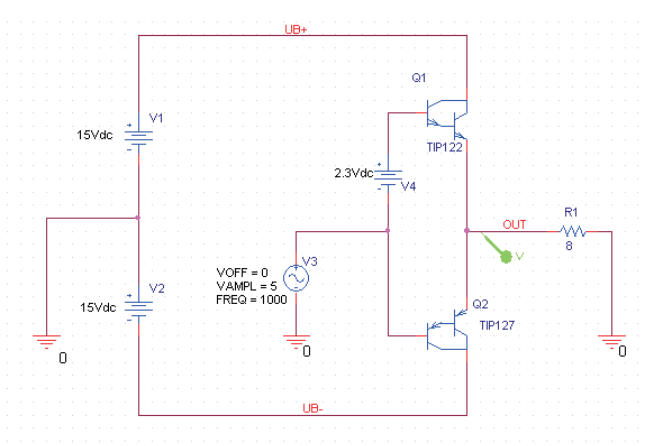
\includegraphics{tex/7_Leistungsverstaerker/pictures/Endstufe_Vorspannung_Schaltung.png}
    \caption{Endstufe mit Vorspannung}
    \label{fig:my_label}
\end{figure}

Wie bereits im Praktikumsskript thematisiert besteht in dieser Schaltung ein Trade-Off zwischen Linearität in der Verstärkung, dem Klirrfaktor und der Verlustleistung. Diese Verlustleisutngen treten nicht nur in den Transistoren, sondern auch im verwendeten Lautsprecher auf. Bei entsprechender Vorspannung erhält das Ausgangssignal einen DC-Offset, auch im Leerlauf wird Leistung in den Lautsprechern umgesetzt. Dies müsste durch eine Koppelkapazität behoben. 

\begin{table}[H]
    \centering
    \begin{tabular}{|c||c|c|}\hline
         $V_4$ & Total Harmonic Distortion & Querstrom im Leerlauf  \\ \hline \hline
         \SI{0}{\volt} (Referenz)& $11.33\%$ & \SI{32}{\micro \ampere} \\ \hline
         \SI{0.7}{\volt}& $7.39\%$ & \SI{32}{\micro \ampere} \\ \hline
         \SI{1.4}{\volt}& $3.54\%$ & \SI{199}{\micro \ampere} \\ \hline
         \SI{2.8}{\volt}& $0.06\%$ & \SI{1.4}{\ampere} \\ \hline
    \end{tabular}
    \caption{verhalten bei verschiedenen Bias-Spannungen}
    \label{tab:my_label}
\end{table}

\section{Der in Brücke geschaltete Verstärker}